
\section{Genomförande}
I följande kapitel redovisas viktiga beslut, förändringar och anpassningar som gjorts 
i projektmetod, projektpraktiker, värderingar, beslut mm som gjorts under studiens genomförande.
(Här kan det vara lämpligt med en indelning i olika ansvarsområden inom projektet?)

\subsection{Projektledning (Stina)}
Genomförandet av iterationer följer helt och hållet mallen för s k ”sprint” i Scrum [ref] 
och beskrivs enklast med följande aktivitetsdiagram, se  bild
\begin{figure}[htbp]
    \centerline{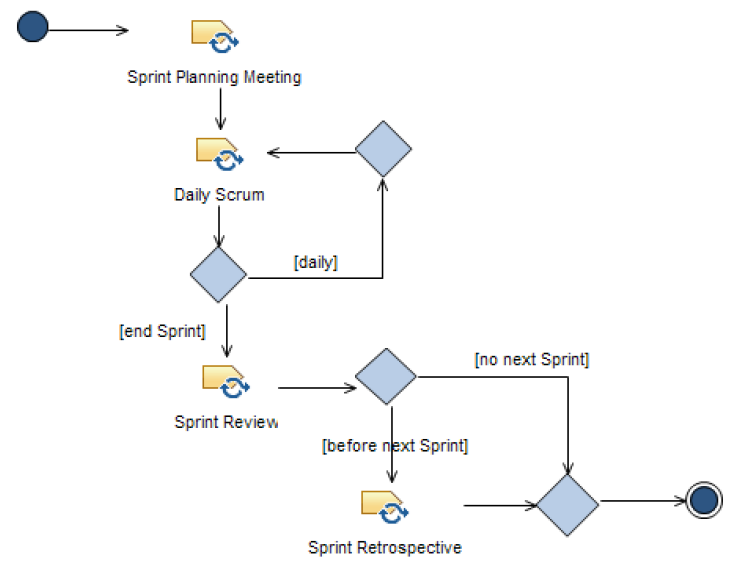
\includegraphics[max height=250px, max width=250px]{images/sprint.png}}
    \caption{Iteration/Sprint}
    \label{fig}
\end{figure}

\subsection{Kundrepresentant (Kurs)}
Lite innehåll.
